%% REGISTRATION NUMBER: 2112102

% SETTING UP
\documentclass[a4paper]{article}
\usepackage{acm,amssymb,amsmath,epsfig,lipsum}
\usepackage[hidelinks]{hyperref}
\setcounter{page}{1}
\sloppy     %line breaks
\ninept

\title{A Review on Text Classification Techniques}

\makeatletter
\def\name#1{\gdef\@name{#1\\}}
\makeatother \name{{\em Registration Number: 2112102}}
\address{\\June 2022 {\small \tt}}


\begin{document}
\maketitle

%ABSTRACT
\begin{abstract}
This paper considers a range of research that utilize various text classification techniques. The major principles in each article are explained in relation to each algorithm, as well as the benefits and drawbacks of each. Machine learning approaches, both supervised and unsupervised, as well as statistical methods like Naive Bayes, are one of these methods.
 \end{abstract}
\noindent{\bf \textit{Keywords}}:\textit{ text classification, algorithm, machine learning, deep learning, statistical methods.}


% INTRODUCTION
\section{Introduction}
Unstructured text is organised into a collection of given categories using text categorization, a machine learning technique. The categories can be chosen ahead of time. Almost any type of data, including digital text, articles, clinical science, and documents, may be managed, arranged, and categorised by content classifiers. \cite{ES1}. For Example, New articles, might be categorized by subject, request for guidance might be prioritized, conversation / interactions can be organized by language, and on and on.

The research of emotions, the identification of topics, the recognition of malware, and the detection of purposes are all uses of text categorization, which is an important aspect of natural language processing (NLP). Words analysis transforms human language to a collection of numbers, providing data structure to make pattern recognition easier. To the extent that the information is well organized, the analysis and conclusions derived from it will be highly accurate. \cite{ES2}. Manually categorising and analysing every little piece of information is equally difficult.
Intelligent text processing techniques for lexical and linguistic pattern analysis have emerged in the natural language processing (NLP).

Text analysis largely depends on a variety of organisational strategies, such as clustering, classification, and categorization. The activity of associating a resource with a specific class label is an excellent example of the above. \cite{ES3}.As a result, text classification is an important step in the process of acquiring knowledge.

The purpose of this report is to give the reader a thorough understanding of the different information retrieval possibilities by looking at the many text classification algorithms which are being used nowadays, the scope to which these algorithms had also expanded along a spectrum of applications, the benefits and challenges of such algorithms.


% BASIC TEXT CLASSIFICATION METHODS
\section{Basic Methods in Text Classification}
among all the different methods which can be used in text classification, these are the main three methods:
\begin{enumerate}
\item Machine Learning
\item Rule-based Systems
\item Hybrid Systems
\end{enumerate}

\subsection{Machine Learning}
A text categorization system which learns to generate categories using machine learning methods does, by learning from past observations. When labelled data are being used as training data for the algorithms (i.e., text), machine learning algorithms might well be capable of understanding the numerous relationships between text segments and the reality that a certain output (i.e., tags) is expected for an input data. \cite{ES4}. A "tag" is a preset category or classification that lets any text to be added to it.

Feature extraction is the initial stage in training a machine learning neural language processing (NLP) classifier, and it involves transforming each line of text into a vector-based numerical representation. \cite{ES5}. The bag of words method is among the most commonly employed techniques. A vector indicates the number of times a specific word occurs in a specified vocabulary of phrases in this approach.

Text classification algorithms in machine learning include:

\subsubsection {Naive Bayes}
	According to a paper by Raschka \cite{ES6},The idea of posterior probabilities is used in a framework to categorise data. \textbf{Baye's Rule}. This is the procedure of categorising and analysing text, and among the most commonly used statistical algorithm groups is the Naive Bayes family. He also proposes the Multinomial Naive Bayes (MNB) technique, a component of this group that gives excellent outcomes regardless of the reality that the set of data is limited and just some few computational materials are available.
The Naive Bayes technique computes the conditional probability of two occurrences by basing the calculation on the probabilities of each individual event. This approach is underpinned by Bayes' Theorem. Determine the chance that each tag applies to the provided text, and then print the tag that has the highest likelihood. The model follows:

\[P(A|B) = \frac{P(A|B)\times P(A)}{P(B)}\]

according to the above equation, Raschka claims that each and every textual vectors would hold data about the presence of text in distinct categories Given additional text criteria.  \cite{ES6}, we can also write the above distribution as:

$$Posterior Probability = \frac{Conditional Probability \times prior probability}{evidence}$$The concept of naive Bayes classification is based on Bayes' theorem, which acts as its core. The posterior probability may be phrased as "What really is the possibility that a specific item fits to the a class given its recorded attribute values?" in the context of a classification issue. (How likely is it when a provided item fits to a class based on its recorded feature values?) This paper also includes a standard technique of \textbf{\textit{Tokenization}}, describing the breakdown of text into tokens.

\subsubsection{Support Vector Machine (SVM)}
Saigal and Khanna used SVM to classify news text \cite{ES7}. They use a hybrid approach in their analysis, combining many techniques.Even before SVM model could start delivering right output, it requires only a small amount of training data. SVM, on the other hand, requires more processing power than Naive Bayes but generates results which are both more quicker and accurate. SVM splits a space into two sub-spaces by forming a line (hyper - plane). Vectors (tags) belonging to one group take up locations inside one plane, whilst vectors belonging in other group take up a position in a different plane. The hyper - plane that provides the greatest outcomes, as shown in Figure 1, is the one that leaves the most space between each tag. Because this approach is multidimensional, more the complicated text data, the accurate the results.

\begin{figure}[tb]
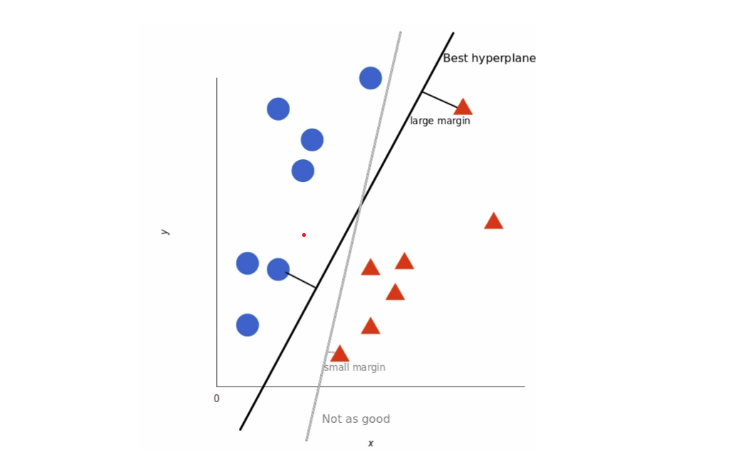
\includegraphics[width=1\columnwidth]{img1.png}
\caption{{\it Support Vector Machine optimal hyperplane. Source: \cite{ES3}}}
\label{spprod}
\end{figure}

The vectors reflect the text data training set, with groups being a tag. The two hyper - planes, according to Saigal and Khanna, are represented by two models:

$$
x^{T} w_{1}+b_{1}=0
$$
and
$$
x^{T} w_{2}+b_{2}=0
$$
where $w_{i}$, $i = [1,2]$ is the normal vector of each hyperplane and $b_{i}$ the bias \cite{ES7}. By reducing the two, the classifier is been produced. The actions they propose are depicted in Figure 2 below.

\begin{figure}[tb]
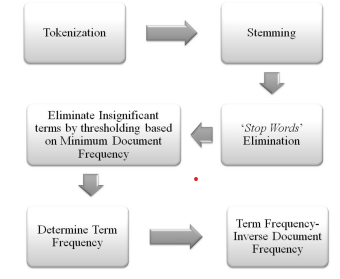
\includegraphics[width=1\columnwidth]{img2.png}
\caption{{\it Pre-processing a text data to perform SVM. Source: \cite{ES7}}}
\label{spprod}
\end{figure}

\subsubsection{Deep Learning}
Deep learning is vital in text classification, as per Guo, who has applied it in sentiment analysis. \cite{ES8}. The recognition of sentiments expressed via written text is largely a classification issue guided by a set of rules and integrating natural language processing (NLP) and deep learning concepts. As a result, he added a talk about deep learning aided in semantic text analysis (DLSTA) for big data-driven human emotion recognition in his work.

Deep learning is a phrase that refers to a collection of tactics and processes which are focused on how neural networks works inside the human brain. Because of their remarkable performance in low-level engineering and execution, deep learning architectures give a variety of advantages for text classification. Convolutional neural networks (CNN) and recurrent neural networks (RNN) are the two most basic forms of deep learning architectures for identifying textual information. Deep learning is a sub-branch of machine learning which includes the sequential execution of a large number of distinct algorithms. Similar to how the human brain comes to decisions by assessing enormous volumes of data in several distinct ways at the same time. Traditional machine learning algorithms require a substantially less amount of training data than deep learning approaches. By developing highly accurate word vector representations, deep learning algorithms are often utilized to improve the performance of classic machine learning classification algorithms. This is accomplished through the development of more precise word vector representations.


\subsection{Rule-Based Techniques}
Rule-based techniques use a set of specific linguistic rules to arrange text into a hierarchy of ordered categories. The machine is encouraged to apply these concepts to find suitable classes related to the content of a text by utilising conceptually relevant text fragments. Every principle has an antecedent (formerly referred as a pattern) as well as a predicted class associated with that too. Rule-based systems that are understandable by humans continue to advance this approach, on either side it has a few drawbacks. A large level of domain expertise is necessary to have these platforms up and operating. They also require a lot of time because developing rules for a complex system can be difficult at times and typically necessitates a huge amount of research and experimenting. Because introducing new rules could possibly modify the consequences of rules which have previously been enforced, rule-based systems are difficult to update and maintain.

\subsection{Hybrid Systems}
Hybrid method combines a fundamental classifier acquired through machine learning with the rule-based approach to achieve superior outcomes. Additional rules for clashing tags, which the basic classifier might have not fully specified, but it can be simply added to these hybrid systems.

% ADVANCED METHODS OF TEXT CLASSIFICATION
\section{Advanced Methods of Text Classification}
The most prevalent text classification methods were reviewed in task 2. More sophisticated approaches not covered above have been explored in this section, including:

\begin{itemize}
    \item K-Nearest Neighbors (KNN) Based Algorithm.
    \item Hierarchical Clustering Algorithm.
\end{itemize}

Because KNN and TF-IDF, as well as Hierarchical Methods and Clustering, are implemented in these techniques, the hybrid-based system is used in each of them.

\subsection{KNN Algorithm}
Trstenjak et al. use the KNN and TF-IDF algorithms to categorise text data. \cite{ES9}. The intention of their Approach is to provide a classification and assessment of how similar two texts are depending on a text sample. It is composed of a number of distinct modules that help consumers with the classification procedure. The Framework is developed in the C Sharp programming language and is deployed in an object-oriented development platform (OOP).

The methodology is based on the assumption that documents may be categorized as points in Euclidean space. The distance that may be measured between two points in Euclidean space is referred to as the Euclidean distance.

\subsubsection{Advantages of KNN Algorithm}

\begin{enumerate}
    \item There is no need to invest time in training (Instance based learning). There are no instructions offered during the training period. Using the training data, no effort has been made to create discriminative functions. To put it differently, prior experience in any manner is not necessary. It retains all training data and only uses it for one purpose: to make real-time predictions for improvement. As a result, KNN is significantly faster than other training-based methods like SVM and Linear Regression.
    
    \item Since the KNN algorithm doesn't really require training to begin producing predictions, additional information may be fed into the system without affecting its performance.
    
    \item The KNN algorithm is a quite simple one. The only two variables required for the design of KNN are K and a distance function (e.g. Euclidean or Manhattan)
\end{enumerate}

\subsubsection{Disadvantages of KNN Algorithm}
\begin{enumerate}
    \item When it comes to dealing with huge data sets, KNN performs quite poorly. Due to the extremely costly nature of calculating the distance between each new point and each old point in massive data sets, the effectiveness of the method is severely hindered.

    \item KNN fails miserably whenever it comes to coping with large amounts of data. The method's usefulness is significantly hampered by the exceedingly expensive nature of computing the distance among every new point and each old point in big data sets.
    
    \item KNN is susceptible to data with noise, missing data, and outliers. The efficiency of the KNN method may be harmed by noise in the given data. Any missing numbers must be manually imputed, and any outliers inside the dataset must be removed.
\end{enumerate}


\subsection{Hierarchical Clustering}
Ranganathan brought this approach to the test in the context of online chat text analysis. \cite{ES10}. According to Ranganathan, "flat text categorization" analyzes categories separately but does not give a framework that explains their relationships. Every new document is assigned to one of the basic categories that seem to be currently available that used a single, massive classifier. Hierarchical text classification employs the divide-and-conquer strategy to successfully execute such a large categorization challenge. Using the hierarchical subject architecture as the foundation for his technique, he designed a method for breaking down the classification task into the number of smaller issues, one per node in the classification tree. A content can be categorised into one or more subcategories for each tier of the category hierarchy through using any of a variety of alternative flat categorization methods. The present level its predecessors and successors can be used to train the classifier.

An article is obtained depending on a keyword combination and matching characteristics, according to the approach employed in this study. The next step is indexing, which entails classifier training and index collection. \cite{ES10}. A specific number of sample articles for every concept are acquired and combined throughout the classifier's training. Pre-processing and indexing are subsequently applied to the resulting of super-documents. Each training set's core acts as a tangible representation of the topic being taught. New articles are indexed using a vector space algorithm to make a traditional word-based index while indexing the collections. This is accomplished while the indexing procedure is in progress. Later that, the document is classified based on the research findings of a correlation of its vector to the notion's center of gravity. The concept-based index which was developed holds the estimated similarity values.


% REFERENCES
\eightpt
\bibliographystyle{IEEEtran}
\begin{thebibliography}{10}

\bibitem[1]{ES1} Baharudin, Baharum \& Lee, Lam Hong \& Khan, Khairullah \& Khan, Aurangzeb. (2010). A Review of Machine Learning Algorithms for Text-Documents Classification. Journal of Advances in Information Technology. 1. 10.4304/jait.1.1.4-20. 

\bibitem[2]{ES2} Amir Gandomi, Murtaza Haider, "Beyond the hype: Big data concepts, methods, and analytics, International Journal of Information Management,"
Volume 35, Issue 2, 2015, Pages 137-144, ISSN 0268-4012, 
https://doi.org/10.1016/j.ijinfomgt.2014.10.007. (https://www.sciencedirect.com/science/article/pii/S0268401214001066)

\bibitem[3]{ES3}   Kobayashi, V. B., Mol, S. T., Berkers, H. A., Kismihók, G., \& Den Hartog, D. N. (2018). Text Classification for Organizational Researchers: A Tutorial. Organizational Research Methods, 21(3), 766–799. https://doi.org/10.1177/1094428117719322

\bibitem[4]{ES4} Dasari, D.B., \&  Rao, G.K. (2012). Text Categorization and Machine Learning Methods: Current State of the Art. Global Journal of Computer Science and Technology Software \& Data Engineering., 12(11), 36-46.

\bibitem[5]{ES5} Gasparetto, A.; Marcuzzo, M.; Zangari, A.; Albarelli, A. A Survey on Text Classification Algorithms: From Text to Predictions. Information 2022, 13, 83. https://
doi.org/10.3390/info13020083

\bibitem[6]{ES6} Raschka, S., (2014). Naive Bayes and Text Classification: Introduction and Theory.  Online: https://sebastianraschka.com/Articles/2014\_naive\_bayes\_1.html

\bibitem[7]{ES7} Saigal, P., Khanna, V., (2020). "Multi‑category news Classification using Support Vector Machine based Classifiers." https://link.springer.com/content/pdf/10.1007/s42452-020-2266-6.pdf

\bibitem[8]{ES8} Guo, J. (2022). Deep learning approach to text analysis for human emotion detection from big data. Journal of Intelligent Systems, 31(1), 113-126. https://doi.org/10.1515/jisys-2022-0001

\bibitem[9]{ES9} Trstenjak, B., Mikac, S., Donko, D., (2014). "KNN with TF-IDF Based Framework for Text Categorization."  Procedia Engineering: 24th DAAAM International Symposium on Intelligent Manufacturing and Automation, 2013, 69(2014 1356-1364

\bibitem[10]{ES10} Ranganathan, S., (2020). "Text Classification Combining Clustering and Hierarchical." University of Madras, Chennai. https://citeseerx.ist.psu.edu/viewdoc/download?doi=10.1.1.135.7298 \&rep=rep1\&type=pdf Approaches 
\end{thebibliography}
\end{document}
